\section{Evaluation}
\label{sec:exp}

Unless
stated otherwise, every method draws from the same candidate frames, sampled from each video at 1 fps and kept at
their native resolution, and receives the same budget of 12,288 tokens per question. \name scores the relevance of each frame with SigLIP~2~\cite{siglip2} and of each transcript segment with
BGE~\cite{bge}, using the question together with its answer options as the query. \name fits $\tau$ on a validation split of each benchmark, which we create when the benchmark provides none, with videos disjoint from the evaluation videos, and keeps it fixed during evaluation. All hyperparameters ($\tau$, $\eta$, $\beta$, $\gamma$, $L$, and the softmax temperature) are tuned on these splits; their values and further implementation details are given in the appendix.

\subsection{Experimental Setup}
\label{sec:exp-setup}

\paragraph{Models.} Qwen3-VL-8B~\cite{bai2025qwen3vl}
encodes each frame at its native resolution, at one token per $32\times32$ pixels, whereas
InternVL3.5-4B~\cite{wang2025internvl35} encodes each $448\times448$ image tile into 256 visual tokens.

\paragraph{Benchmarks.} We use three long-video multiple-choice benchmarks. For MLVU~\cite{zhou2024mlvu}, we use the 2,174 questions of its development set. For LongVideoBench
(LVB)~\cite{wu2024longvideobench}, we use its validation set of 1,337 questions. Neither provides subtitles in our setting, so the input is visual only.
Video-MME~\cite{fu2024videomme} contains 2,700 questions on short, medium, and long videos; we use its subtitled
setting, in which subtitle tokens count toward the same budget. For the multi-turn setting, we use 200 conversations of
MT-Video-Bench (MTVB)~\cite{mtvideobench2025}, whose answers are scored by an LLM judge (Gemini~3.8 Flash); the judge prompt is given in the appendix.

\paragraph{Metrics.} We report accuracy together with compute, measured in TFLOPs per question: the prefill compute
of the language models of all VLMs that a method calls, summed over every call for that question. For conversations,
we sum the compute over all turns. Offline indexing is not counted. We focus on compute and cost rather than latency.

\paragraph{Baselines.} Uniform sampling is the plain VLM with uniformly sampled frames at the same budget. All other methods extend the same embedding-based RAG pipeline, and differ in how they turn its
candidates into the input of the VLM:
\begin{itemize}
  \item Top-K (w/ pruning): Retrieves the top-64 frames by relevance and keeps 192 tokens of each with the token
    pruner of \name. Its frame count is tuned on the validation splits (32 to 256 frames at the same budget), where accuracy varies by less than \simnum{1} point.
  \item Q-Frame~\cite{zhang2025qframe}: Shows frames at three resolutions by relevance rank. We replace its Long-CLIP scorer with SigLIP~2.
  \item QuoTA~\cite{luo2025quota}: Scores each frame with a small VLM after decoupling the question, and assigns
    each frame a number of tokens that grows with its score.
  \item FOCUS~\cite{zhu2026focus}: Selects keyframes from short clips by bandit exploration.
  \item AdaAlloc~\cite{an2026adaalloc}: Lets the VLM plan how to split the budget between sparse low-resolution
    frames and dense high-resolution frames (concurrent work).
\end{itemize}
Every baseline receives the same candidate frames and, on Video-MME, the same retrieved transcript segments, and each
reimplementation matches the published accuracy of its method in the original setting.
Graph-based RAG is also prevalent in video understanding systems~\cite{ren2025videorag,shen2025vgent,yan2025ava,yang2026g2frag,chen2026memdreamer,yan2026ecrag}. We therefore also pair \name with VideoRAG~\cite{ren2025videorag}, whose retrieved frames \name re-allocates under the same budget.

\subsection{Main Results}
\label{sec:exp-main}

\begin{table*}[t]
  \centering
  \small
  \renewcommand{\arraystretch}{1.08}
  \newcommand{\group}[1]{\rowcolor{groupbg}\multicolumn{10}{l}{\textit{#1}} \\}
  \newcommand{\maintab}{%
  \begin{tabular}{l cc cc ccccc}
    \toprule
    \multirow{2}{*}{Method} & \multicolumn{2}{c}{MLVU (w/o subtitles)} & \multicolumn{2}{c}{LVB (w/o subtitles)} & \multicolumn{5}{c}{Video-MME (w/ subtitles)} \\
    \cmidrule(lr){2-3} \cmidrule(lr){4-5} \cmidrule(lr){6-10}
    & Overall~$\uparrow$ & TFLOPs~$\downarrow$
      & Overall~$\uparrow$ & TFLOPs~$\downarrow$
      & Overall~$\uparrow$ & Short~$\uparrow$ & Medium~$\uparrow$ & Long~$\uparrow$
      & TFLOPs~$\downarrow$ \\
    \specialrule{\lightrulewidth}{\aboverulesep}{0pt}
    \group{Qwen3-VL-8B~\cite{bai2025qwen3vl}}
    Uniform sampling & \cellcolor{heat4}\simnum{72.8} & \cellcolor{heat1}\simnum{216} & \cellcolor{heat4}\simnum{61.9} & \cellcolor{heat1}\simnum{231} & \cellcolor{heat4}\simnum{71.2} & \cellcolor{heat3}\simnum{80.9} & \cellcolor{heat4}\simnum{70.8} & \simnum{61.9} & \cellcolor{heat1}\simnum{229} \\
    RAG                                                      & & & & & & & & & \\
    \quad + Top-K (w/ pruning) & \cellcolor{heat3}75.9 & \cellcolor{heat1}218 & \cellcolor{heat3}64.0 & \cellcolor{heat1}232 & \cellcolor{heat4}73.1 & \cellcolor{heat2}82.4 & \cellcolor{heat3}73.4 & 63.6 & \cellcolor{heat1}230 \\
    \quad + Q-Frame~\cite{zhang2025qframe}\venue{ICCV'25} & \cellcolor{heat3}74.7 & \cellcolor{heat1}209 & \cellcolor{heat2}65.7 & \cellcolor{heat1}225 & \cellcolor{heat4}71.1 & \cellcolor{heat3}80.1 & \cellcolor{heat4}70.3 & 63.0 & \cellcolor{heat0}218 \\
    \quad + QuoTA~\cite{luo2025quota}\venue{AAAI'26} & \cellcolor{heat2}77.2 & 781 & \cellcolor{heat1}66.6 & 676 & \cellcolor{heat3}74.4 & \cellcolor{heat1}83.2 & \cellcolor{heat3}74.4 & \cellcolor{heat4}65.4 & 647 \\
    \quad + FOCUS~\cite{zhu2026focus}\venue{ICLR'26} & \cellcolor{heat4}71.7 & \cellcolor{heat1}211 & \cellcolor{heat3}64.0 & \cellcolor{heat1}226 & \cellcolor{heat4}70.1 & \cellcolor{heat4}79.1 & \cellcolor{heat4}69.4 & 61.8 & \cellcolor{heat1}224 \\
    \quad + AdaAlloc~\cite{an2026adaalloc}\venue{NeurIPS'26} & \cellcolor{heat4}73.2 & \cellcolor{heat0}203 & \cellcolor{heat3}65.1 & \cellcolor{heat0}222 & \cellcolor{heat4}71.0 & \cellcolor{heat1}82.8 & \cellcolor{heat4}69.4 & 60.7 & \cellcolor{heat1}225 \\
    \quad + \textbf{\name (Ours)} & \cellcolor{heat1}78.1 & \cellcolor{heat2}230 & \cellcolor{heat1}66.6 & \cellcolor{heat1}234 & \cellcolor{heat1}77.3 & \cellcolor{heat0}\textbf{83.6} & \cellcolor{heat1}76.8 & \cellcolor{heat1}71.7 & \cellcolor{heat1}232 \\
    VideoRAG~\cite{ren2025videorag} & \cellcolor{heat3}\simnum{76.4} & \cellcolor{heat2}\simnum{226} & \cellcolor{heat3}\simnum{65.2} & \cellcolor{heat1}\simnum{238} & \cellcolor{heat3}\simnum{74.0} & \cellcolor{heat1}\simnum{82.6} & \cellcolor{heat3}\simnum{74.3} & \cellcolor{heat4}\simnum{65.1} & \cellcolor{heat1}\simnum{236} \\
    \quad + \textbf{\name (Ours)} & \cellcolor{heat0}\textbf{\simnum{78.6}} & \cellcolor{heat2}\simnum{233} & \cellcolor{heat0}\textbf{\simnum{67.3}} & \cellcolor{heat1}\simnum{239} & \cellcolor{heat0}\textbf{\simnum{77.6}} & \cellcolor{heat1}\simnum{83.4} & \cellcolor{heat0}\textbf{\simnum{77.1}} & \cellcolor{heat0}\textbf{\simnum{72.3}} & \cellcolor{heat1}\simnum{237} \\
    \specialrule{\lightrulewidth}{0pt}{0pt}
    \group{InternVL3.5-4B~\cite{wang2025internvl35}}
    Uniform sampling & \cellcolor{heat4}\simnum{69.8} & \cellcolor{heat1}\simnum{146} & \cellcolor{heat4}\simnum{58.6} & \cellcolor{heat1}\simnum{146} & \cellcolor{heat4}\simnum{65.6} & \cellcolor{heat3}\simnum{75.6} & \cellcolor{heat4}\simnum{65.3} & \simnum{55.9} & \cellcolor{heat1}\simnum{143} \\
    RAG                                                      & & & & & & & & & \\
    \quad + Top-K (w/ pruning) & \cellcolor{heat3}\simnum{72.5} & \cellcolor{heat1}\simnum{147} & \cellcolor{heat3}\simnum{60.4} & \cellcolor{heat1}\simnum{147} & \cellcolor{heat4}\simnum{67.7} & \cellcolor{heat2}\simnum{77.3} & \cellcolor{heat3}\simnum{68.1} & \simnum{57.8} & \cellcolor{heat1}\simnum{144} \\
    \quad + Q-Frame~\cite{zhang2025qframe}\venue{ICCV'25} & \cellcolor{heat3}\simnum{71.3} & \cellcolor{heat0}\simnum{141} & \cellcolor{heat2}\simnum{62.1} & \cellcolor{heat0}\simnum{142} & \cellcolor{heat4}\simnum{65.7} & \cellcolor{heat4}\simnum{75.0} & \cellcolor{heat4}\simnum{65.0} & \simnum{57.2} & \cellcolor{heat0}\simnum{136} \\
    \quad + QuoTA~\cite{luo2025quota}\venue{AAAI'26} & \cellcolor{heat3}71.3 & 708 & \cellcolor{heat2}62.5 & 583 & \cellcolor{heat4}64.9 & \cellcolor{heat4}74.7 & \cellcolor{heat4}64.6 & 55.4 & 551 \\
    \quad + FOCUS~\cite{zhu2026focus}\venue{ICLR'26} & \cellcolor{heat4}69.5 & \cellcolor{heat1}142 & \cellcolor{heat4}58.8 & \cellcolor{heat1}143 & \cellcolor{heat4}66.4 & \cellcolor{heat3}75.9 & \cellcolor{heat4}65.9 & 57.4 & \cellcolor{heat1}140 \\
    \quad + AdaAlloc~\cite{an2026adaalloc}\venue{NeurIPS'26} & \cellcolor{heat3}71.1 & 314 & \cellcolor{heat0}\textbf{63.6} & 331 & \cellcolor{heat4}67.9 & \cellcolor{heat0}\textbf{79.2} & \cellcolor{heat4}66.7 & 57.8 & 325 \\
    \quad + \textbf{\name (Ours)} & \cellcolor{heat0}\textbf{\simnum{74.7}} & \cellcolor{heat1}\simnum{155} & \cellcolor{heat1}\simnum{63.0} & \cellcolor{heat1}\simnum{148} & \cellcolor{heat0}\textbf{\simnum{72.0}} & \cellcolor{heat1}\simnum{78.5} & \cellcolor{heat0}\textbf{\simnum{71.5}} & \cellcolor{heat0}\textbf{\simnum{65.9}} & \cellcolor{heat1}\simnum{145} \\
    \specialrule{\heavyrulewidth}{0pt}{\belowbottomsep}
  \end{tabular}}%
  \sbox0{\setlength{\tabcolsep}{0pt}\maintab}%
  \setlength{\tabcolsep}{\dimexpr(\textwidth-\wd0)/20\relax}%
  \maintab
  \caption{\textbf{Main results.} Accuracy (\%) on MLVU, LongVideoBench (LVB), and Video-MME with subtitles at a
    budget of 12,288 tokens, with the compute (TFLOPs per question) of each method on each benchmark. Within each VLM
    block, darker cells are closer to the best value of their column, and the best accuracy is in bold.}
  \label{tab:main}
\end{table*}

\paragraph{\name achieves the Pareto frontier in single-turn question answering.}
\cref{tab:main} compares all methods at the budget of 12,288 tokens. With Qwen3-VL-8B and embedding-based RAG, \name
attains the highest accuracy on all three benchmarks, tied with QuoTA on LVB. At matched compute, it exceeds Q-Frame, FOCUS, and AdaAlloc by 0.9 to 7.2 points. Relative to Top-K (w/ pruning),
\name gains 2.2, 2.6, and 4.2 points on MLVU, LVB, and Video-MME. The gain is largest on the long videos of Video-MME (8.1 points), where the relevant evidence is sparse. QuoTA is the closest baseline: its difference to \name on MLVU and LVB is within one point and not significant (paired McNemar test, $p\ge0.12$),
but its per-frame scorer calls cost 2.8--3.4$\times$ more compute. The gains carry over to
InternVL3.5-4B: \name remains the most accurate method on MLVU and
Video-MME, where it improves on the best baseline by \simnum{2.2} and \simnum{4.1} points, and is within
\simnum{0.6} points of AdaAlloc on LVB at less than half of its compute. \name also transfers to graph-based retrieval: paired with VideoRAG, it gains
\simnum{2.2}, \simnum{2.1}, and \simnum{3.6} points on the three benchmarks at about the same compute.

\cref{fig:budget} and \cref{fig:multiturn}(a) vary the budget from 1,536 to 12,288 tokens on MLVU. \name is the most
accurate method at every budget, and its advantage grows as the budget shrinks: at 1,536 tokens it reaches 73.4\%, 8.3 points above Top-K (w/ pruning). With 3,072 tokens (53 TFLOPs), it exceeds the accuracy of Q-Frame,
FOCUS, and AdaAlloc at 12,288 tokens (203--211 TFLOPs), a reduction of nearly 4$\times$.

\begin{figure}[t]
  \centering
  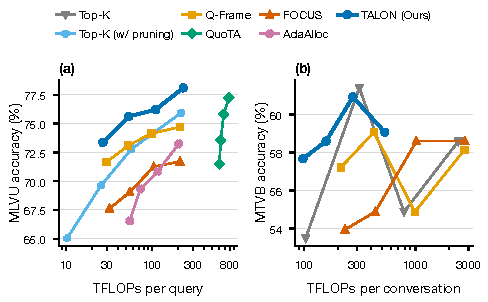
\includegraphics[width=\linewidth]{fig/tflops_pair.pdf}
  \caption{\textbf{Accuracy against compute.} (a)~Single turn: MLVU accuracy against TFLOPs per query.
    (b)~Multi turn: MT-Video-Bench accuracy (a 100-conversation subset for the four-budget sweep, 215 judged turns) against TFLOPs per conversation, summed over all turns. Each line spans per-turn budgets from 1,536 to 12,288 tokens.}
  \label{fig:multiturn}
\end{figure}

\paragraph{\name achieves the Pareto frontier across multi-turn conversations.}
\cref{fig:multiturn}(b) reports accuracy against the compute of a whole conversation on MT-Video-Bench. All methods keep the KV cache across turns, and a baseline skips a frame that the cache already holds at the selected
resolution. The baselines still add the new frames of every question, whereas \name prefills only the tokens that the
cache lacks. At the same
per-turn budget, it consequently uses 2.2--5.2$\times$ less compute than Q-Frame and FOCUS and up to 4.6$\times$ less
than Top-K (w/ pruning), and it is the most accurate method at three of the four budgets. A turn after the first finds a median of 81\% of its tokens already in the cache
(\cref{fig:overlap}(b)).

\begin{table}[t]
  \centering
  \small
  \renewcommand{\arraystretch}{1.2}
  \settowidth{\splitw}{Medium}%
  \newcommand{\abltab}{%
  \begin{tabular}{l@{\hspace{5pt}} c VVVV}
    \toprule
    Method & TFLOPs $\downarrow$
      & \multicolumn{4}{c}{%
        \begin{tabular}{@{}VVVV@{}}
          \multicolumn{4}{c}{Video-MME (w/ subtitles) $\uparrow$} \\
          \cmidrule(lr){1-4}
          Overall & Short & Medium & Long \\[2.6pt]
        \end{tabular}} \\
    \specialrule{\lightrulewidth}{\aboverulesep}{0pt}
    \textbf{\name} & \cellcolor{heat1}232 & \cellcolor{heat0}\textbf{77.3} & \cellcolor{heat0}\textbf{83.6} & \cellcolor{heat0}\textbf{76.8} & \cellcolor{heat0}\textbf{71.7} \\
    \hspace{0.5em}w/o water-filling & \cellcolor{heat1}\simnum{229} & \cellcolor{heat3}\simnum{74.8} & \cellcolor{heat1}\simnum{83.4} & \cellcolor{heat1}\simnum{76.0} & \cellcolor{heat4}\simnum{64.9} \\
    \hspace{0.5em}w/o text allocation & \cellcolor{heat0}226 & \cellcolor{heat3}73.7 & \cellcolor{heat2}81.9 & \cellcolor{heat2}74.9 & \cellcolor{heat4}64.4 \\
    \hspace{0.5em}w/o diversity & \cellcolor{heat0}226 & \cellcolor{heat1}76.6 & \cellcolor{heat2}82.4 & \cellcolor{heat1}76.4 & \cellcolor{heat1}70.8 \\
    \bottomrule
  \end{tabular}}%
  \sbox0{\setlength{\tabcolsep}{0pt}\abltab}%
  \setlength{\tabcolsep}{\dimexpr(\columnwidth-\wd0)/11\relax}%
  \xdef\ablsep{\the\tabcolsep}%
  \abltab
  \caption{\textbf{Ablation of the Token Scheduler} on Video-MME with subtitles (Qwen3-VL-8B, 12,288 tokens). Each
    row removes one component of \name.}
  \label{tab:ablation}
\end{table}

\paragraph{Performance breakdown.}
\cref{tab:ablation} removes one component of the Token Scheduler at a time. Replacing water-filling with an
allocation proportional to relevance, at matched compute, lowers accuracy by \simnum{2.5} points overall and by
\simnum{6.8} points on long videos. Removing text allocation, so that each shown frame only brings its time-aligned subtitles, costs 3.6 points overall and 7.3 points on long videos. Removing the
diversity term costs 0.7 points. The vision encoder runs once per video, at 48 TFLOPs, and its output is reused across questions and turns.

\cref{tab:multiturn} ablates the two multi-turn components at 6,144 tokens per turn. Updating relevance with the
attention of the VLM improves accuracy by 1.1 points and reduces compute by 13\%, since attention concentrates the
allocation on frames that the cache already holds. Without the carried allocation, every turn recomputes its evidence
from scratch, which raises compute by \simnum{2.3}$\times$ with no gain in accuracy; appending tokens thus costs no accuracy. A sensitivity analysis of the
hyperparameters is given in the appendix.

\begin{table}[t]
  \centering
  \small
  \renewcommand{\arraystretch}{1.2}
  \setlength{\tabcolsep}{\ablsep}%
  \settowidth{\dimen0}{\hspace{0.5em}w/o carried allocation}%
  \dimen2=\dimexpr(\columnwidth-5\tabcolsep-5pt-\dimen0)/2\relax
  \begin{tabular}{l@{\hspace{5pt}} >{\centering\arraybackslash}p{\dimen2} >{\centering\arraybackslash}p{\dimen2}}
    \toprule
    Method & TFLOPs $\downarrow$ & MTVB (w/o subtitles) $\uparrow$ \\
    \midrule
    \textbf{\name} & \cellcolor{heat0}275 & \cellcolor{heat0}\textbf{58.5} \\
    \hspace{0.5em}w/o attention & \cellcolor{heat2}315 & \cellcolor{heat2}57.4 \\
    \hspace{0.5em}w/o carried allocation & \simnum{640} & \cellcolor{heat1}\simnum{58.2} \\
    \bottomrule
  \end{tabular}
  \caption{\textbf{Ablation of multi-turn scheduling} on MT-Video-Bench (Qwen3-VL-8B; 200 conversations, 450 judged turns; 6{,}144
    visual tokens per turn). TFLOPs are summed over all turns of a conversation.}
  \label{tab:multiturn}
\end{table}
